\documentclass[a4paper]{book}

\usepackage{blindtext}
\usepackage[dutch]{babel}
\usepackage[top=2.5cm, left=2.5cm, bottom=2.5cm, right=2.5cm]{geometry}
\usepackage[colorlinks=true, breaklinks]{hyperref}
\usepackage[round,authoryear]{natbib}
\usepackage{graphicx}
\usepackage{enumerate}

\usepackage{xcolor}
\definecolor{c1}{rgb}{0,0,1} % blue
\definecolor{c2}{rgb}{0,0.3,0.9} % light blue
\definecolor{c3}{rgb}{0.3,0,0.9} % red blue
\hypersetup{
    linkcolor={c1}, % internal links
    citecolor={c2}, % citations
    urlcolor={c3} % external links/urls
}

\addto\extrasdutch{  
	\def\chapterautorefname{Hoofdstuk}  
	\def\sectionautorefname{Sectie}  
	\def\figureautorefname{Figuur}  
	\def\tableautorefname{Tabel}  
}

\begin{document}

\selectlanguage{dutch}

\title{Latex voor beginners}
\author{Bas de Reus}
\date{\today}
\maketitle
\tableofcontents

\chapter{Basis}

\blindtext
\blindtext

\section{Voorbeeld Sectie}

\blindtext

\subsection{Voorbeeld Subsectie}

\blindtext

\subsubsection{Voorbeeld Sub-subsectie}

\blindtext

%##noBuild
\chapter{Opsommingen}
\label{opsomming}

\section{Opsomming met nummering}

\blindtext

1,2, \ldots

\begin{enumerate}
  \item Eerste item
  \item Tweede item
\end{enumerate}

\blindtext

a, b, \ldots

\begin{enumerate}[a)]
  \item Eerste item
  \item Tweede item
\end{enumerate}

\blindtext

1,2, \ldots voorafgegaan met 3 spaties en gevolgd door een afsluitende haak   

\begin{enumerate}[~~~1)]
  \item Eerste item
  \item Tweede item
\end{enumerate}

\blindtext

\section{Opsomming zonder nummering}

\blindtext

\begin{itemize}
  \item Eerste item
  \item Tweede item
\end{itemize}

\blindtext

\chapter{Verwijzingen}
\label{hyperlinks}

\blindtext[7]

\label{page_hyperlinks}

\section{Sectie verwijzing}
\label{sectie_hyperlinks}

\blindtext[7]

\section{Refs}

Hyperlink met alleen nummer \ref{hyperlinks}.  
Nummer zonder hyperlink \ref*{hyperlinks}

\section{Autorefs}

\autoref{hyperlinks}
\autoref{sectie_hyperlinks}

\section{Hyperrefs}

\hyperref[hyperlinks]{Aangepaste versie \ref*{hyperlinks}}

\section{Voetnoten}

\blindtext

Met dank aan\footnote{voetnoot tekst}

\blindtext

\section{Urls}

Internet links \url{https://ctan.org}
of \href{https://ctan.org}{CTAN website}

\section{Literatuur verwijzingen}

Cite \cite{Martin2018}

en

Citep \citep{Martin2018}

\chapter{Afbeeldingen}
\label{afbeeldingen}

\section{Importeren afbeelding}

\blindtext

\begin{figure}[h!]
	\centering
	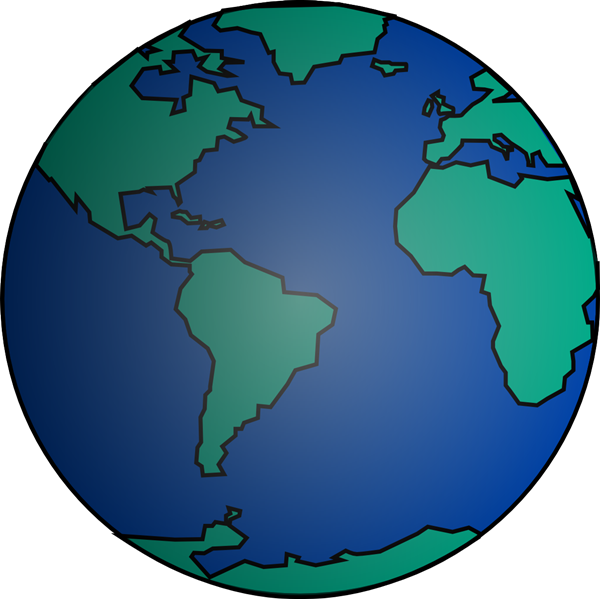
\includegraphics[width=0.3\textwidth]{boek-bestanden/aarde}
	\caption{Aarde}
	\label{aarde}
\end{figure}

\blindtext

\autoref{aarde}
%##noBuild
\chapter{Tabellen}
\label{tabellen}

\section{Tabel}

\blindtext

\begin{table}[h!]
	\begin{tabular}{lr}
	cel (1,1)
	& cel (1,2)
	\\
	cel (2,1)
	& cel (2,2)
	\end{tabular}
\end{table}

\blindtext

\begin{table}[h!]
	\label{tabel}
	\centering
	\begin{tabular}{|l|c|l|}
	\hline
	
	& kop 1
	& kop 2
	\\ \hline
	rij 1
	& cel (1,1)
	& cel (1,2)
	\\
	rij 2
	& cel (2,1)
	& cel (2,2)
	\\ \hline
	\end{tabular}
	\caption{Tabel Verwijzing}
\end{table}

\blindtext

\autoref{tabel}


\bibliographystyle{abbrvnat}
\bibliography{boek-bestanden/library}

\listoffigures
\listoftables

\end{document}